%\mbox{}
%\thispagestyle{empty}

\thispagestyle{plain}
\section{Anchor systems}
An anchor is a steel element either cast into concrete or post-installed into a hardened concrete member and used to transmit applied loads, including headed bolts, hooked bolts (J- or L-bolt), headed studs, expansion anchors, or undercut anchors \cite{anchors-ACI-318M}. Anchors are typically used to connect structural elements or to fix non-structural components (or systems) to the structures. 

\begin{figure}[h!]
	\centering
	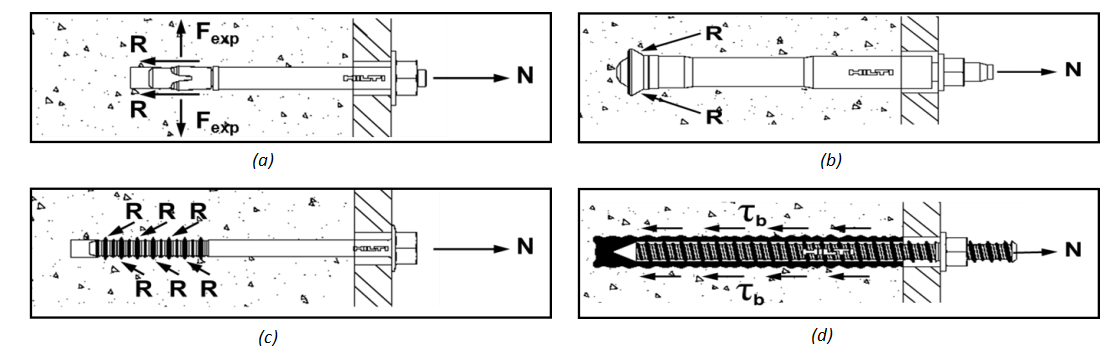
\includegraphics[width=0.9\textwidth]{obrazky/post_installed_anchor_types_repaired.png}
	\caption[Types of post-installed anchors with different load transfer mechanism]{Categorizing of post-installed anchors by load transfer mechanism ($R$ is direction of reaction force, $N$ is loading of anchor and $F_{exp}$ represent expansion force) \cite{hilti_anchors}: a) friction (micro-keying); b) keying (bearing/undercut); c) keying (screw-type); d) adhesion (bonding).}\label{obr:Post_installed_anchors}
\end{figure}

\subsection{Load transfer mechanisms}
In the Fig. \ref{obr:Post_installed_anchors} we can see different types of load transfer mechanisms. The choice of a  used mechanism affects future method of installation, resilience to different types of loading and even curing time, which some anchors need before loading. Each anchor type is described below in detail. 


\begin{itemize}
	\item \textit{Friction mechanism}
	As the name implies, the primary transfer mechanism is friction and it results in bonding from expansion forces between the anchor and the primary structure (Fig. \ref{obr:Post_installed_anchors}a). Frictional force is proportional to the magnitude of expansion stresses generated by the anchor.The expansion is caused by a controlled torque during casting and even, in some cases, later adjusted for changes in the state of the base material.
	
	\item \textit{Keying mechanism}
	This transfer principle rely on the interlock of the anchor with deformations in the hole wall to resist external loading (Fig. \ref{obr:Post_installed_anchors}b,c). The bearing stresses created in the base material in the interface with the anchor bearing surface can rise to high levels due to the triaxial nature of the stress state. This type of anchors offers good resilience to variations in the base material conditions and thus represent one of the most robust solution for most anchor designs. 
	
	\item \textit{Bonding mechanism}
	This mechanism relies on adhesion between the concrete and the anchor created by adhesive (Fig. \ref{obr:Post_installed_anchors}d). The degree of bonding available is depending on the condition of the hole wall at the time of anchor installation and used type of adhesive material. This type of mechanism offers flexibility and high bond resistance for a wide variety of anchoring applications. 
\end{itemize}

\begin{figure}[h!] 
	\centering 
	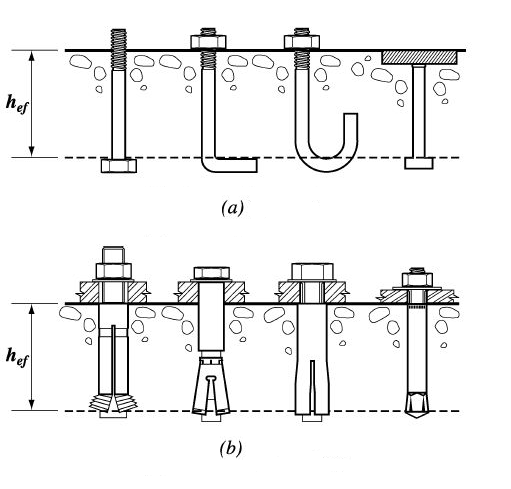
\includegraphics[width=0.6\textwidth]{obrazky/anchor_types_repaired.png} 
	\caption[Types of anchors]{Types of anchors ($h_{ef}$ is effective anchor length) \cite{anchors-ACI-318M}: a) cast-in-place; b) post-installed.}\label{obr:Anchors} 
\end{figure} 


\newpage
\subsection{Types of anchors}
\indent

Anchors can be divided by the load transfer mechanism, but another important criterion before choosing a specific solution is the installation time, when an anchor is fixed. As you can see in Fig. \ref{obr:Anchors}, anchors can be divided into two main groups: $\mathrm{a)}$ cast-in-place and $\mathrm{b)}$ post-installed. 


\subsubsection{Cast-in-place anchors}
The cast-in-place anchors are the simplest type of anchor. As the name suggests, these anchors are cast in the wet concrete or with reinforcement of concrete. In the Fig. \ref{obr:Anchors} we can see that most designs consist of a standard bolt with a hexagonal head (hex head bolt $\mathrm{(b.1)}$), though there are other designs such as “hooked” J bolts  $\mathrm{(b.2)}$ and L bolts $\mathrm{(b.3)}$. These anchors are very strong, and can be used in most anchor applications, but they are also difficult to cast. Therefore, they are recommended when the large embedment length or the  high tensile strength are required.

\subsubsection{Post-installed anchors}
Post-installed anchors are in general, technically sophisticated products, but are easy to install and provide more variability than cast-in anchors like headed studs. They can be cast into already harden concrete as well as into masonry but they are a lot more sensitive to the boundary conditions than cast-in anchors. Most of the commercially available anchor products can be assigned to one of the major types which are categorized according to their load transfer mechanism (Fig. \ref{obr:Post_installed_anchors}).


\subsubsection{Types of post-installed anchors}
Four main groups of post-installed anchors based on a load transfer mechanism and method of installation can be found in the literature \cite{hilti_anchors}.
 
	\begin{itemize}

	\item Expansion anchors. Primary principles of load transfer are friction, bearing or both. Anchors are inserted into a drilled hole in the hardened concrete or masonry. Main advantages are immediate load transfer and no temperature restrictions, but on the other hand they are not the best in transfer capacity. 

	\item Undercut anchors create holding strength due to the mechanical interlock provided by undercutting the concrete near the back of the hole. This is achieved by a special tool or by the anchor itself during installation. The main load transfer method is keying. This type of anchors have benefits like high transfer capacity, immediate loading transfer, or no temperature restrictions, but they are more difficult to install. 

	\item Screw anchors are inserted into drilled hole with a diameter typically smaller than the anchor. Typical load transfer mechanism is keying. The advantages are immediate full loading transfer or no temperature restrictions, but the anchors can reach just low loading capacity.

	\item Adhesive anchors are post-installed into drilled hole in hardened concrete, masonry or stone. Loads are transferred to the base material by the bond created by an adhesive on the anchor, so the load transfer mechanism is a bonding. Advantages of this type of anchor are a simple installation and a high capacity, main disadvantages are temperature restrictions and a curing time needed before loading, or the anchor would be damaged. But full curing state is not typically reached. Modeling partly cured adhesive is difficult due to a large number of variables such a loading history, time, temperature, even humidity. Modeling of this adhesive material is the main target of this thesis.
\end{itemize} 

\subsection{Loading and failure modes}
An anchor is in most cases loaded in tension and shear. This loading checks all parts of anchor, even the base material. According to a norm \cite{anchors-ACI-318M}, the strength design of anchors shall be based either on computation using design modes that satisfy requirements of the norm, or on test evaluation using the 5 percent fractile of test results for the following:

\begin{itemize}
	\item steel strength of anchor in tension,
	\item steel strength of anchor in shear, 
	\item concrete breakout strength of anchor in tension,
	\item concrete breakout strength of anchor in shear,
	\item pullout strength of anchor in tension (including adhesive), 
	\item concrete side-face blowout strength of anchor in tension,
	\item concrete pry out strength of anchor in shear.
\end{itemize} 

\begin{figure}
	\centering
	\begin{subfigure}{.5\textwidth}
		\centering
		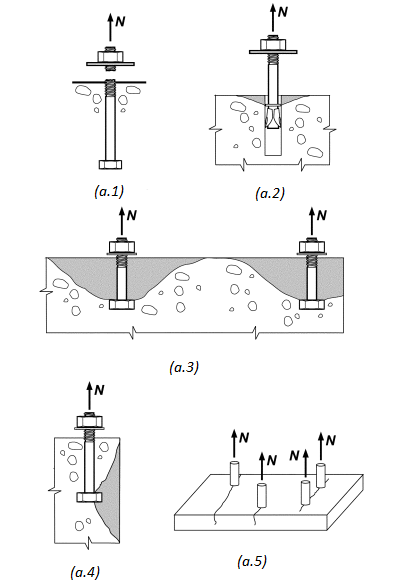
\includegraphics[width=.9\linewidth]{obrazky/failure_models_tensile.png}
		\caption{tensile loading, where $N$ is tensile force}
		\label{obr:tensile_loaded}
	\end{subfigure}%
	\begin{subfigure}{.5\textwidth}
		\centering
		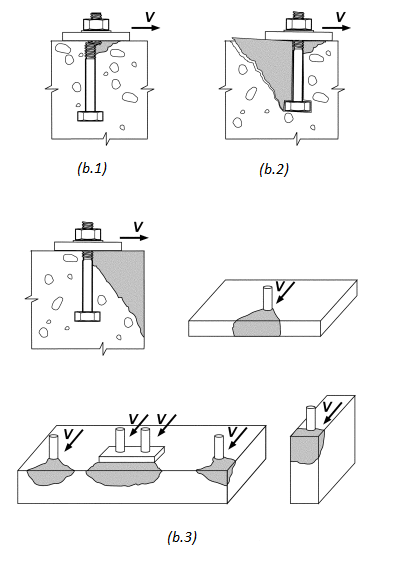
\includegraphics[width=.9\linewidth]{obrazky/failure_models_shear.png}
		\caption{shear loading, where $V$ is shear force}
		\label{obr:shear_loaded}
	\end{subfigure}
	\caption[Failure modes of anchors]{Failure modes of anchors \cite{anchors-ACI-318M}: a.1) steel failure; a.2) pullout; a.3) concrete breakout; a.4) side-face blowout; a.5) concrete splitting; b.1) steel failure preceded by concrete spalling; b.2) concrete pryout for anchors far from a free edge; b.3) concrete breakout.}
	\label{obr:failture_models}
\end{figure}


\begin{figure}[h!]
	\centering
	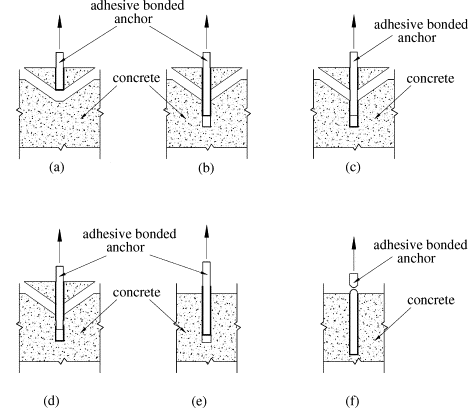
\includegraphics[width=0.6\textwidth]{obrazky/adhesive_failture_models_repaired.png}
	\caption[Failure modes of adhesive anchors in tensile]{Failure modes of adhesive anchors in tension \cite{adhesive_anchors}: a) concrete cone failure; b) adhesive/concrete interface bond failure; c) steel/adhesive interface bond failure; d) mixed bond failure; e) bond failure; f) steel failure.}
	\label{obr:failture_adhesive_models}
\end{figure}
 
These failure modes are shown in Fig. \ref{obr:failture_models}. However, adhesive anchors have even more complicated failure modes due to a full length bond, which can be damaged in different ways, see Fig. \ref{obr:failture_adhesive_models}.
